\chapter{Background}\label{chap:background}
In this chapter we will briefly introduce some basic model definitions and notation conventions for the following chapters.

\section{Basic Model Definitions and Notations}\label{sec:backgroundBasic}
A Setup $A$ is defined by
\begin{itemize}
    \item a set $S$ of $M$ Sources: $S=\{S_1,S_2,...,S_M\}$,
    \item a set $R$ of $N$ Receivers: $R=\{R_1,R_2,...,S_N\}$,
    \item a set $Q$ of $K$ Obstacles: $Q=\{Q_1,Q_2,...,Q_K\}$ and
    \item a tuple of physical properties: $(\vartheta,\phi, p)$
\end{itemize}
where
\begin{conditions}
    M           & number of source nodes, $M \in \mathbb{N}$ \\
    N           & number of receiver nodes, $N \in \mathbb{N}$ \\
    K           & number of obstacles, $K \in \mathbb{N}$ \\
    \vartheta   & temperature in $[^{\circ}\textrm{C}]$ \\
    \phi        & relative humidity, $\phi \rightarrow [0, 1]$ \\
    p           & atmospheric pressure in $[\textrm{Pa}]$
\end{conditions}

An Environment $E$ is defined by
\begin{itemize}
    \item a set $Q$ of $K$ Obstacles: $Q=\{Q_1,Q_2,...,Q_K\}$ and
    \item a tuple of physical properties: $(\vartheta,\phi, p)$
\end{itemize}

Therefore a Setup $A$ can also be described by
\begin{itemize}
    \item a set of $M$ Sources: $\{S_1,S_2,...,S_M\}$,
    \item a set of $N$ Receivers: $\{R_1,R_2,...,S_N\}$ and
    \item an Environment $E$
\end{itemize}

\section{Spherical Coordinates}
For the spherical coordinates, in particular the spherical angles, the \emph{mathematical} convention as shown in \figref{fig:spherical} will be used.
\begin{figure}[H]
    \begin{center}
    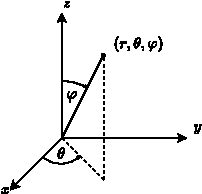
\includegraphics[width=\textwidth/2]{figures/background/spherical.pdf}
    \end{center}
    \caption[Spherical Coordinates]{Spherical Coordinates}
    \label{fig:spherical}
\end{figure}

where
\begin{conditions}
    r       & radial distance, $r \rightarrow \mathbb{R}$ \\
    \theta  & azimuthal angle, $\theta \rightarrow (-\pi, \pi]$ \\
    \varphi & polar angle, $\varphi \rightarrow [0, \pi]$
\end{conditions}
